\documentclass[landscape, a4paper]{article}
\usepackage[margin=0cm,top=0.4cm,bottom=0.4cm,left=0.4cm,right=0.4cm]{geometry}
% \usepackage[showframe,margin=0cm,top=0.5cm,bottom=0.5cm,left=0.5cm,right=0.5cm]{geometry}
\usepackage[export]{adjustbox}
\usepackage{xcolor}
\usepackage{caption}
\usepackage{csquotes}
\usepackage{titlesec}
\usepackage{etoolbox} % Add this to your preamble
\usepackage[parfill]{parskip}

\newtoggle{isEnglish}
\toggletrue{isEnglish}
% \togglefalse{isEnglish}

\captionsetup{labelformat=empty, justification=centering, font={color=PrimaryColor}}

\definecolor{PrimaryColor}{HTML}{5B632A} % Tyrian purple
\newcommand\alert[1]{\textcolor{PrimaryColor}{\textbf{#1}}}

\titleformat{\section}
{\color{PrimaryColor}\normalfont\normalsize\bfseries}
{\thesection}{0.5cm}{}
\titlespacing{\section}{0cm}{0.2cm}{0.2cm}
% \renewcommand{\thesection}{\arabic{section}}

\titleformat{\subsection}
{\color{PrimaryColor}\normalfont\normalsize\bfseries}
{\thesubsection}{0.5cm}{}
\titlespacing{\subsection}{0cm}{0.1cm}{0.1cm}

\begin{document}
\noindent
\centering
\footnotesize
\begin{minipage}[t]{0.31\textwidth}
	\setlength{\parskip}{0.25cm}
	\vspace{0.5cm}

	\textcolor{PrimaryColor}{
		\rule{\linewidth}{0.5mm}
		\vspace{-0.1cm}
		\begin{center}
			\large
			\textsc{\iftoggle{isEnglish}{Hike to the Forest Sanctuary St. Odile}{}}
		\end{center}
		\rule{\linewidth}{0.5mm}
	}

	\iftoggle{isEnglish}{
    Our journey begins at the \alert{\enquote{Stadtgarten} (city garden)}, established in 1888 as part of an ambitious urban development plan following Freiburg’s industrial growth and the increasing popularity of public green spaces across Germany. Its design was influenced by the ideals of the English landscape garden, with winding paths, a pond, and gently rolling lawns. Until 1911, it even required an entrance fee. 

    This green oasis has evolved into both a cherished public park and a living museum of horticultural (cultivation of gardens and plants for decorative or practical use) and arboricultural (care and management of trees and shrubs) richness. The Stadtgarten is known for its rose gardens, including up to 250 varieties of roses, which can be found in the countless flower beds.% which was originally planted in the 1920.

    % A key feature is the cable car station at the edge of the park, from which the Schlossbergbahn funicular railway has been operating since 2008, offering visitors a direct route to the Schlossberg’s panoramic viewpoints.
	}{
	}

	\includegraphics[width=\linewidth]{./figures/stadtgarten.png}
	\captionof{figure}{\iftoggle{isEnglish}{\enquote{Stadtgarten} (city garden) with schlossberg tram}{}}
	\setlength{\parskip}{0.25cm}

	\iftoggle{isEnglish}{
    % Botanically, the Stadtgarten is home to many trees and shrubs offering a remarkable blend of native and exotic flora. . %which features heritage rose varieties and seasonal plantings.% that attract pollinators. Since the 1980s, ecological gardening practices have been emphasized, including the planting of wildflower meadows and the maintenance of habitats for birds, bees, and small mammals.
    % Among them are sequoias, ginkgos, Japanese cherry trees, silver limes, and magnolias, many of which were planted during the park’s formative decades. Several specimens, including some giant sequoias (Sequoiadendron giganteum), date back to the 1890s, making them over 130 years old today. 

		Our trip continues to the \alert{\enquote{Schlossberg} (castle hill)}, the towering hill that rises to the east of Freiburg’s \enquote{Altstadt} (old town), offering not only stunning panoramic views of the city and the Rhine Valley, but also a deep and complex history stretching back over a thousand years.

		In 1091, \alert{Berthold II of Zähringen}, Duke of Swabia and founder of Freiburg, constructed a fortress on the Schlossberg. This castle, known as the Castellum de Friburch, was the power base for the Zähringer family and gave Freiburg its name: \enquote{frei Burg} meaning \enquote{free castle}.

		% The castle's location allowed the Zähringers to control key trade routes through the Black Forest and the Dreisam Valley. The original castle was likely a mix of stone and timber structures, fairly modest by later standards, but it was formidable for its time.
		After the Zähringers died out in 1218, the castle passed to the \alert{Counts of Urach}, later known as the Counts of Freiburg, and eventually to the Habsburgs, who ruled the region for centuries.
	}{
	}
\end{minipage}%
\hfill%
\vrule width 0.01cm
\hfill%
\begin{minipage}[t]{0.31\textwidth}
	\vspace{0cm}
	\setlength{\parskip}{0.25cm}

	\iftoggle{isEnglish}{
	}{
		In the 17th century, during the Thirty Years’ War, the Schlossberg again became a focal point for military strategy. Recognizing its importance, the \alert{French} under Louis XIV had their star military engineer, Sébastien Le Prestre de Vauban, build a massive baroque fortress on the hill when they captured Freiburg in the late 1600s.
	}

	\includegraphics[width=\linewidth]{./figures/rosskopf_resized.png}
	\captionof{figure}{\iftoggle{isEnglish}{\enquote{Schlossberg} (castle hill) and behind it \enquote{Roßkopfberg} (horse head mountain)}{}}
	\setlength{\parskip}{0.25cm}

	\iftoggle{isEnglish}{
		% The Schlossberg, \enquote{literally Castle Hill}, has always held strategic importance due to its elevation and its commanding view over the surrounding region. Archaeological evidence suggests that the hill was used for fortified settlements as early as the Bronze Age, but its most significant period began in the 11th century.
		\alert{Sébastien Le Prestre de Vauban (1633–1707)} was a brilliant French military engineer and Marshal of France under King Louis XIV. Vauban is widely regarded as one of the greatest minds in military architecture, revolutionizing fortification design during the age of gunpowder.

		Vauban’s hallmark was his distinctive \alert{star-shaped fortress system}, designed to withstand and repel the increasing power of cannon fire, which had made traditional medieval walls obsolete. Instead of relying on high vertical walls, which could be easily destroyed by artillery, Vauban used low, angled ramparts to deflect cannonballs, Bastions and zigzag-shaped outer defenses to eliminate blind spots and allow overlapping fields of fire, moats, earthworks, and tunnels to absorb shock and delay attackers.

		Freiburg came under French occupation in 1677 during the Franco-Dutch War, and Vauban was ordered to transform the city into a modern fortress at the edge of French-controlled territory.

		From 1679 to 1681, and again after another French occupation in 1744, he oversaw the construction of an enormous fortress complex on the Schlossberg and redesigned the city’s defenses to match his cutting-edge military theories.

		After the \alert{Treaty of Ryswick in 1697}, Freiburg reverted to Austrian control, and the French were forced to destroy the fortifications in 1745 during the War of the Austrian Succession. They did so thoroughly: the entire fortress was blown up with explosives, and much of what remained was later quarried for building stone.
		% Though most of the fortress was blown up in 1745 during France's withdrawal (as required by treaty), the legacy of Vauban’s work remains etched into the landscape and memory of Freiburg—especially on the Schlossberg, where remnants of his fortifications are still visible.

		In the 1990s, Freiburg took a bold step in urban planning and named a new sustainable district after the famed engineer. The Vauban district, located on the site of a former French military base (used after World War II), became a model eco-neighborhood when development began in 1998.

		On the Schlossberg, we're going to see a lot of interesting sights that bring Freiburg’s rich history, scenic beauty, and local culture to life. From former fortifications to memorials, fountains, and lookout points, each stop reveals a unique story.
	}{
	}
\end{minipage}%
\hfill\color{white}%
\vrule width 0.01cm
\hfill\color{black}%
\begin{minipage}[t]{0.31\textwidth}
	\vspace{0cm}
	\setlength{\parskip}{0.25cm}

	\iftoggle{isEnglish}{
		No full structures remain from the Zähringer castle or Vauban fortress, but you can still find ruins of fortification walls and one can visit the \alert{\enquote{Kanonenplatz} (cannon plaza)}. This iconic terrace was once part of the French artillery positions during Freiburg’s occupation under Louis XIV. Named “Cannon Plaza”, it offers a panoramic view over the Old Town and was first fortified during the 1670s, when Vauban built the city’s massive defensive system
		% , a scenic overlook that once held French artillery. 
	}{
	}

	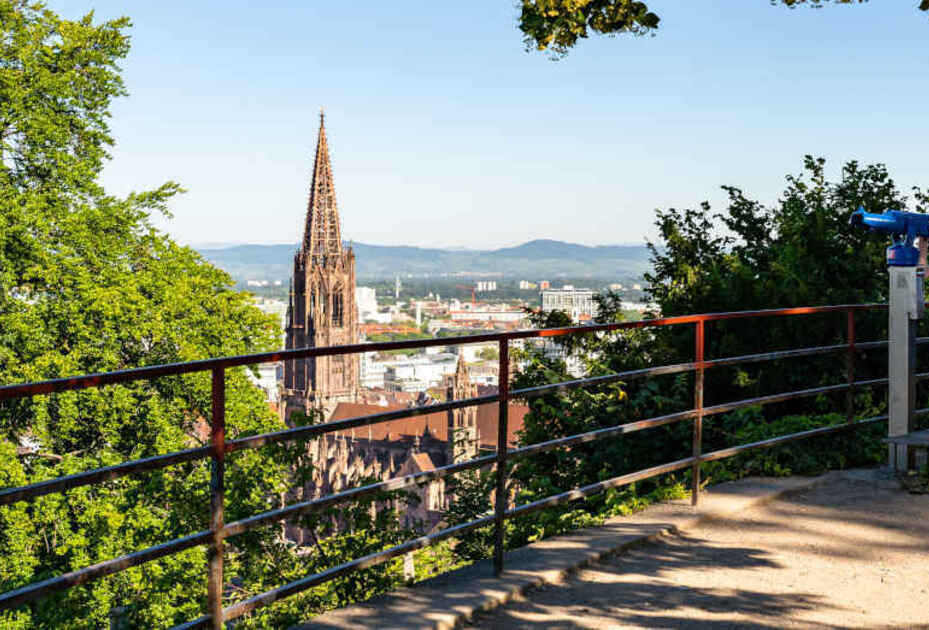
\includegraphics[width=\linewidth]{./figures/kanonenplatz_resized.png}
	\captionof{figure}{\iftoggle{isEnglish}{\enquote{Kanonenplatz} (cannon plaza)}{}}
	\setlength{\parskip}{0.25cm}

	\iftoggle{isEnglish}{
		Installed in 2017 an interactive marble run called \alert{\enquote{Schlossberg Kugelbahn}} is a modern attraction for children and families. It winds creatively along the hillside using wood and steel tracks, letting visitors roll large wooden balls down the slope. %It playfully blends modern design with the natural landscape.

    The \alert{\enquote{Kommandantengarten} (commandant's barden)} is a serene terrace nestled on the western slope of the Schlossberg. Its name harks back to its historical role as the private garden of the fortress commandant during the era when Freiburg's Schlossberg was a strategic military stronghold. %Today, it offers visitors a tranquil setting with panoramic views over Freiburg's Altstadt, making it a favored spot for both relaxation and reflection.

    % Perched atop the Schlossberg lies the Fort Carré, a testament to 17th-century military engineering. Constructed under the direction of French military architect Sébastien Le Prestre de Vauban during the French occupation of Freiburg, this square fortification featured bastions at each corner and served as the final defensive retreat for the fortress commandant in times of siege. Although much of the original structure was dismantled in the 18th century, remnants remain, offering insights into the fort's formidable design

    Tucked into the summit of Freiburg’s Schlossberg lies the historic \alert{Fort Carré}, a striking example of 17th-century military engineering. Built during the French occupation of Freiburg under the direction of renowned military architect Sébastien Le Prestre de Vauban, the fort formed part of an elaborate system of defenses constructed between 1677 and 1681. The name \enquote{Fort Carré} is French and translates literally to \enquote{square fort} (fort meaning fortification and carré meaning square or quadrilateral). This designation reflects the fort’s original geometric layout, a compact square plan with bastions at each corner. It is a hallmark of Vauban’s fortress style, designed to maximize defense and minimize blind spots. Strategically placed as the last redoubt or fallback position, Fort Carré served as the commandant’s final point of retreat in the event of siege.

		There’s also a metal viewing tower, the \alert{\enquote{Schlossbergturm} (castle hille tower)}, built in 2002 and 35 meters tall, that gives a 360-degree view over Freiburg, the Black Forest, and even the Vosges mountains in France on a clear day.
		% Built in 2002, the Schlossberg Tower stands 35 meters tall and was designed by architect Jürgen Grossmann. Constructed using local larch wood and steel, it stands on the site of former military signal towers and offers a 360-degree view—stretching from the Black Forest to the Vosges mountains.
%     The Kleine Kanonenplatz (Small Cannon Square) is a modest terrace situated along the eastern slope of the Schlossberg, en route to the St. Ottilien Chapel. While less prominent than its larger counterpart, the Kanonenplatz, this site holds its own historical significance.
%
% The name "Kleine Kanonenplatz" reflects its historical use as a smaller artillery position during the period when the Schlossberg was fortified. These fortifications were part of the extensive military structures developed over the centuries, particularly during the times when the Schlossberg served as a strategic defense point for Freiburg.
	}{
	}
\end{minipage}%
\newpage
\begin{minipage}[t]{0.31\textwidth}
	\vspace{0cm}
	\setlength{\parskip}{0.25cm}

	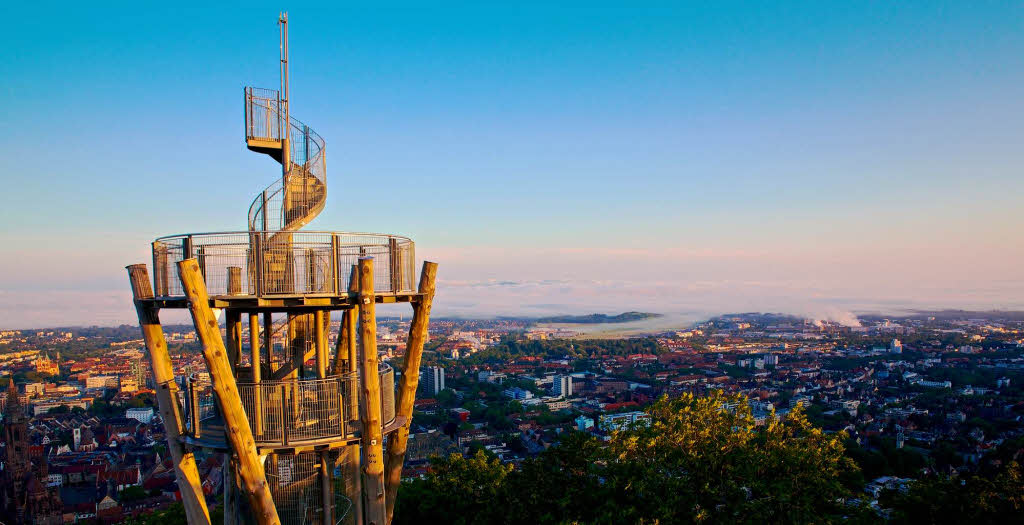
\includegraphics[width=\linewidth]{./figures/schlossbergturm.png}
	\captionof{figure}{\iftoggle{isEnglish}{\enquote{Schlossbergturm} (castle hill tower)}{}}
	\setlength{\parskip}{0.25cm}

	\iftoggle{isEnglish}{
		From the Schlossberg, our journey continues to the \alert{Roßkopf}, a prominent peak in the Black Forest just northeast of Freiburg’s city center. With an elevation of 737 meters above sea level, the Roßkopf stands as one of the highest points near the city, offering expansive views over the Rhine Valley, the Kaiserstuhl hills, and on clear days, even to the Vosges Mountains in France.

		The name Roßkopf translates literally to \enquote{horse’s head}. It likely stems from the mountain’s rounded summit, which was said to resemble the shape of a horse's head when viewed from the surrounding valleys. The term "Roß" is an old German word for horse.%, emphasizing the area's long-standing connection to traditional rural life.

		One of the most striking modern features of the Roßkopf summit is a set of four \alert{large wind turbines}, installed in 2003 and each standing about 98 meters tall and each producing clean electricity for approximately 3,000 households.%, they were among the first citizen-funded wind energy projects in Baden-Württemberg.%The turbines produce renewable electricity for thousands of households and symbolize Freiburg’s commitment to sustainability.
	}{
	}

	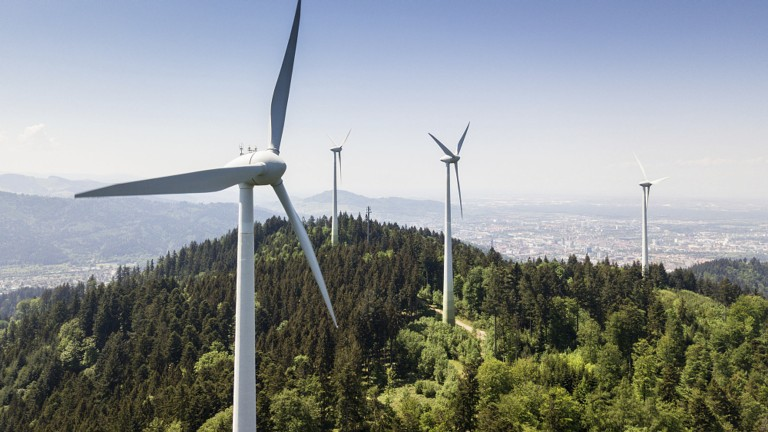
\includegraphics[width=\linewidth]{./figures/windpark-rosskopf_pic_768.jpg}
	\captionof{figure}{\iftoggle{isEnglish}{Wind turbines on top of the Roßkopf}{}}
	\setlength{\parskip}{0.25cm}

	\iftoggle{isEnglish}{
		Another major highlight is the \alert{\enquote{Roßkopfturm} (horse head tower)}, a metal observation tower built in 1889. Standing 34.4 meters high, the tower was erected as a monument to regional tourism and nature appreciation. Its steel lattice design, rare for its time, still offers one of the best panoramic viewpoints in the region. It is also known as \enquote{Friedrichsturm}, named in honor of Grand Duke Friedrich I of Baden, a patron of nature conservation and tourism.
 % by the \enquote{Schwarzwaldverein} (Black Forest Association)
	}{
	}

\end{minipage}%
\hfill%
\vrule width 0.01cm
\hfill%
\begin{minipage}[t]{0.31\textwidth}
	\vspace{0cm}
	\setlength{\parskip}{0.25cm}

	\iftoggle{isEnglish}{
		On the way to the Roßkopf, we pass by the \alert{\enquote{Waldrestaurant St. Ottilien} (Forest Restaurant St. Odile)}, a beloved forest eatery nestled amidst the serene woodlands of Freiburg. In April 2025, St. Ottilien faced a significant challenge when a fire broke out in the dishwashing area, causing damage to the kitchen and dining spaces. While the indoor areas are undergoing restoration, the restaurant has partially reopened, serving guests in the outdoor seating area. %A community-led fundraising campaign is underway to support the establishment during this rebuilding phase. Despite these setbacks, the dedicated team at St. Ottilien continues to provide warm hospitality and delicious meals, making it a worthwhile stop on your journey to the Roßkopf.
	}{
  }

	\includegraphics[width=\linewidth]{./figures/friedrichsturm.png}
	\captionof{figure}{\iftoggle{isEnglish}{\enquote{Roßkopfturm} (Roßkopf tower)}{}}
	\setlength{\parskip}{0.25cm}

	\iftoggle{isEnglish}{
    Right next to the Forest Restaurant St. Ottilien lies the \alert{\enquote{Waldheiligtum St. Ottilien} (Forest Sanctuary of St. Ottilien)}, a peaceful place that has drawn pilgrims and locals alike for centuries. The chapel is consecrated to Saint Odile, she is said to have been a 7th-century noblewoman. Born blind, she is believed to have miraculously gained her sight during baptism and has since been venerated as the patron saint of the blind and those with eye ailments. The name St. Odile reflects this connection, in the Middle Ages, a healing spring is said to have emerged near this site in Freiburg’s forest, believed to possess curative powers, especially for eye conditions. %Over time, the site became known as a place of prayer and pilgrimage, particularly among those seeking relief or guidance. The first chapel stood at this place in 679 (in accordance with the information board in the chapel). The spring still flows beside the sanctuary, marked by a stone basin and devotional figures.

    % She is usually depicted with an abbess bar and a book on which two or three eyes are lying, indicating that she was born blind and is believed to cure eye diseases. The church was built over a spring whose water contains radon which is said to alleviate eye diseases. % The forest sanctuaries of St. Odile, St. Wendelin, and St. Valentine, together with the nearby Loretto Chapel, are cherished spiritual sites nestled within Freiburg’s hills.

	}{
	}

	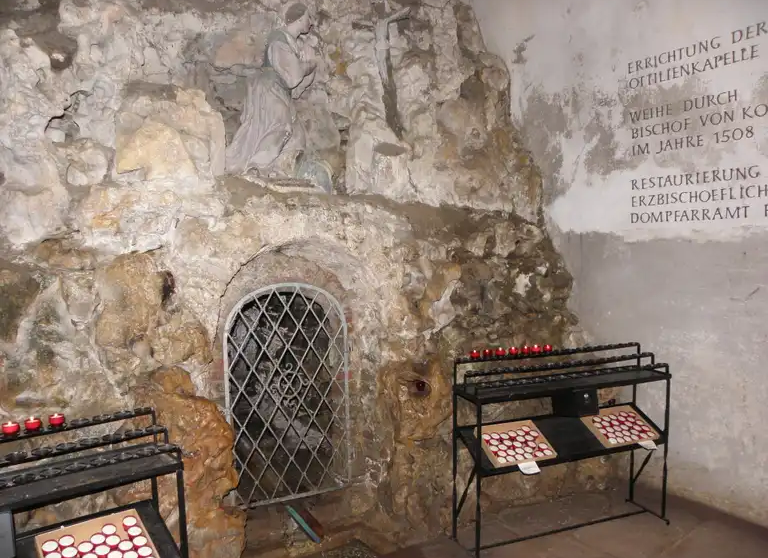
\includegraphics[width=\linewidth]{./figures/waldheiligtum_st_ottilien_resized.png}
  \captionof{figure}{\iftoggle{isEnglish}{\enquote{Waldheiligtum St. Ottilien} (Forest sanctuary St. Odile)}{}}
	\setlength{\parskip}{0.25cm}
\end{minipage}%
\hfill\color{white}%
\vrule width 0.01cm
\hfill\color{black}%
\begin{minipage}[t]{0.31\textwidth}
	\vspace{0cm}
	\setlength{\parskip}{0.25cm}

	\iftoggle{isEnglish}{
		% located at Talstraße 131 in Gundelfingen
    % Descending from the forest sanctuary of St. Odile, we continue our journey down the Roßkopf and arrive in the district of Littenweiler, where the Dreisam River marks the boundary between nature and civilization.
    Descending from the forest sanctuary of St. Odile, we continue down the Roßkopf, cross the clear waters of the Dreisam, and enter the district of \alert{Littenweiler}. First documented in the 11th century as Lutenwile, Littenweiler began as a modest farming village on the eastern outskirts of Freiburg. The village's name reflects its agricultural roots, and over the centuries, it maintained a rural character, with a population comprising farmers and day laborers. In 1914, Littenweiler was incorporated into the city of Freiburg, marking a significant shift in its development.
% , nestled at the edge of the Black Forest where the Dreisamtal opens into the Zartener Becken. 

    The \alert{Dreisam River}, stretching 29.7 kilometers, originates in the Black Forest near Kirchzarten from the confluence of the Rotbach and Wagensteigbach. Its name derives from the Celtic Tragisamā, meaning "the very fast one," reflecting its swift current. Historically, the Dreisam was prone to flooding, with a notable flood in March 1896 causing significant damage in Freiburg. To mitigate such risks, the river was channelized in the late 19th century, with embankments constructed to protect the city. The Dreisam also feeds Freiburg's historic Bächle, the small water-filled runnels that run through the city's old town, adding to its unique charm.

    In Littenweiler, culinary enthusiasts can indulge in diverse dining experiences, such as the Moroccan restaurant Scherazade and the Italian Ristorante Pizzeria Colosseo. The former restaurant pays homage to \alert{Scheherazade}, the sultan's wife who, according to legend, told captivating stories each night to postpone her execution. Through her wit and storytelling, she not only saved her own life but also the lives of many other women. The latter restaurant draws its name from the iconic \alert{Colosseum} in Rome, symbolizing the grandeur of Italian heritage.
 % Scherazade, named after the legendary storyteller of One Thousand and One Nights, offers a taste of Moroccan cuisine. 
	}{
	}

	\includegraphics[width=\linewidth]{./figures/dreisam_littenweiler.png}
	\captionof{figure}{\iftoggle{isEnglish}{The river Dreisam in Littenweiler}{}}
	\setlength{\parskip}{0.25cm}

  Our journey through Freiburg’s storied heights and hidden valleys draws to a close along the banks of the Dreisam in Littenweiler, where the murmuring river marks a quiet return to the city’s edge. From the panoramic Schlossberg and its many historical sights, to the forested slopes of the Roßkopf crowned by the Friedrichsturm, and onward past the forest sanctuary of St. Odile, we’ve walked in the footsteps of dukes, pilgrims, and visionaries. This route through nature and time offers more than just landscapes: it’s a historical roundup, woven with forest paths, fortress stones, and culinary moments.
\end{minipage}%
\newpage
\begin{minipage}[t]{0.31\textwidth}
	\setlength{\parskip}{0.25cm}
	\vspace{0.5cm}

	\textcolor{PrimaryColor}{
		\rule{\linewidth}{0.5mm}
		\vspace{-0.1cm}
		\begin{center}
			\large
			\textsc{Addendum}
		\end{center}
		\rule{\linewidth}{0.5mm}
	}

	\iftoggle{isEnglish}{
		Located near the Kanonenplatz, this war memorial was erected in 1930 to honor the soldiers of the \alert{\enquote{5th Badenisches Feldartillerie-Regiment Nr. 76}}, based in Freiburg and active during World War I. The regiment had a close relationship with the city, and the monument remains a place of remembrance.

		The \alert{\enquote{Ludwigshöhe}}, named after Grand Duke Ludwig I of Baden, this high point on the southern slope of the Schlossberg was laid out in the 19th century as a scenic overlook and picnic area. It offers sweeping views toward the Rhine Valley and the Kaiserstuhl hills. It was part of a romantic landscaping effort to make the hill more accessible for leisure walks.

		The \alert{\enquote{Silberbrunnen} (silver fountain)} lies in a quiet, wooded section of the Schlossberg and dates back to medieval times. It supplied water to both the castle and city below. According to local legend, the name comes from the silvery shimmer of the water or possibly from silver coins found near the spring. Its cool water still flows today.

		There's also the \alert{\enquote{Kleiner Kanonenplatz} (little cannon plaza)}, it's a smaller, lesser-known platform located above the main Kanonenplatz. It offers a more intimate view over the city and was also part of the historic French fortification system built by Vauban in the late 17th century.

		The \alert{Tusculum} is a modest villa-like structure built in the 19th century as a leisure and event house for Freiburg’s educated elite. Named after the ancient Roman retreat town of Tusculum, it was a symbol of cultured urban recreation. Today, it's occasionally used for cultural events and private gatherings.

		The \alert{\enquote{Festung Freiburger Schlossberg}} is a historical trail. This self-guided historical walking route, marked with signs and maps, takes visitors through the remaining fortification structures from the Vauban era and earlier medieval layers. It traces bastions, walls, trenches, and casemates, offering rich context through on-site information boards.

		The \alert{\enquote{Brunnen bei den Siebenlinden}} is a fountain near the Seven Lindens area is named for a group of linden trees that once stood prominently here. The trees were a landmark on the 19th-century romantic walking paths, and the small spring-fed fountain served local hikers and picnic-goers.

		The \alert{\enquote{Katharinenbrunnen} (catherine’s fountain)}, located near the remnants of old fortress walls, was named after Saint Catherine, likely due to a nearby former chapel or shrine. Though modest, it reflects the spiritual and practical significance of water sources on the hill.
	}{
	}
\end{minipage}%
\hfill%
\vrule width 0.01cm
\hfill%
\begin{minipage}[t]{0.31\textwidth}
	\vspace{0cm}
	\setlength{\parskip}{0.25cm}

	\iftoggle{isEnglish}{
		Located near a former forest trail junction, the \alert{\enquote{Husarenbrunnen}} (Hussars’ fountain) is a small spring named after the light cavalry units (Hussars) who are said to have watered their horses here in the 19th century, possibly during Prussian military movements or training exercises in the region.

		The \alert{\enquote{Martinsfelsen}} (Martin’s rock), is a rugged sandstone outcrop located just below the summit plateau of the Roßkopf. It is named after St. Martin, one of the most venerated saints in the region. It may have been a historic waypoint for pilgrims or shepherds, although no formal shrine existed here.


		Our trip begins at the \alert{\enquote{Schwabentor} (swabian gate)}, one of the two remaining medieval city gates of Freiburg im Breisgau. This striking gate, whose name translates to "Swabian Gate," is not just an architectural relic, it's a doorway into centuries of history, legend, and the cultural crossroads of southern Germany.

		The \enquote{Schwabentor} was built around 1250 as part of Freiburg’s second city wall expansion. At the time, Freiburg was growing rapidly, and the city’s leadership recognized the need for better fortifications. The gate stood as both a protective bulwark and a checkpoint for traders and travelers entering the city from the south and southeast, especially from the direction of the Swabian regions which gives the gate its name.
		Perhaps the most captivating feature of the \enquote{Schwabentor} is the large fresco on its inner wall, painted by Fritz Geiges in 1903. It depicts a Swabian merchant who, according to legend, once tried to buy all of Freiburg with a cart full of gold, but when it turned out his \enquote{gold} was just sand-covered rocks, he was laughed out of town.

		This legend, while likely apocryphal, ties into a long-standing rivalry and playful mockery between the people of Baden (where Freiburg is located) and Swabians to the east. Hence, the name \alert{Swabian Gate} could be a mix of historical reference and local humor.


		The \alert{\enquote{Schwabentorsteg} (swabian gate footbridge)} is a covered wooden pedestrian bridge located at the eastern edge of Freiburg’s Old Town. Built in 1970, the bridge spans the Schlossbergring, a four-lane bypass road encircling the historic city center. Measuring approximately 25 meters in length, the Schwabentorsteg blends harmoniously with the historic atmosphere of the Old Town thanks to its traditional wooden construction.

		% Its purpose is to connect Salzstraße, one of Freiburg’s oldest and most charming streets, directly with the Schlossberg, the city's iconic castle hill.
		Nestled between the slopes of the Roßkopf and the Schönberg, the \alert{Wildtal} is a peaceful side valley of the Glottertal, just northeast of Freiburg. Though easily accessible, it retains the charm of a secluded rural landscape with deep roots in the region’s natural and cultural history.

		The name \alert{\enquote{Wildtal}} literally means \enquote{Wild Valley}, and is believed to derive from the abundance of wild animals, especially deer and boar, that once roamed the area. In medieval times, it served as a hunting ground for local nobility and monastic orders. %The name likely also reflects the dense, uncultivated forests that once covered the slopes before extensive clearing began in the Middle Ages.

		%Perched at approximately 478 meters above sea level on a ridge between the Wildtal and Gundelfingen, this castle is considered the ancestral seat of the House of Zähringen, one of the most influential noble families in southwest Germany.
		On the way into the Wildtal, we pass the \alert{Zähringer Castle Ruin} (\enquote{Zähringer Burg}), a site of great historical significance. The original Zähringer Castle was likely constructed around the early 11th century, though the first documented reference appears in 1128. It served as a fortified residence for the Zähringer dukes, who controlled extensive territories across Baden, Switzerland, and parts of Alsace.
	}{
	}
\end{minipage}%
\hfill\color{white}%
\vrule width 0.01cm
\hfill\color{black}%
\begin{minipage}[t]{0.31\textwidth}
	\vspace{0cm}
	\setlength{\parskip}{0.25cm}

	\iftoggle{isEnglish}{
		The \alert{Zähringers} played a decisive role in the founding of Freiburg in 1120, which they developed as a free market city. However, after the extinction of the Zähringer male line in 1218, the castle began to lose its importance. Today, visitors can see the foundation walls, a reconstructed tower (built in 1906), and information panels about the site’s past

		Later as we'll be descending from the Zähringer Castle Ruin, we're going to arrive in the \alert{district of Zähringen}, a part of Freiburg that carries the name and legacy of this southern Germany’s influential noble family.

		% The nearby Forest Restaurant St. Ottilien takes its name from this sacred site. Originally developed as a resting place for pilgrims and hikers, the restaurant honors the area’s history by providing a place of refreshment and hospitality near the sanctuary.

		% On the way to the Zähringen Castle Ruin, we pass by the \alert{Forest Restaurant Zähringer Burg}, a charming woodland eatery nestled at the foot of the historic castle site. This restaurant offers a delightful stop for hikers and history enthusiasts alike. The Forest Restaurant Zähringer Burg is renowned for its regional and seasonal specialties. For those seeking lighter fare or a quick bite, the restaurant offers a selection of snacks and desserts, such as Homemade cakes and Ice cream desserts.
	}{
	}
	\iftoggle{isEnglish}{
    One of its most notable landmarks was the Stadthalle (Festival Hall), completed in 1905 and designed in a neo-baroque style. It served as a prestigious venue for concerts, dances, and civic events. The hall was destroyed in the night of bombing on 27 November 1944 and was not been rebuilt afterwards. Today, the rose garden is situated in the hall's former location.
  }{
  }

	\includegraphics[width=\linewidth]{./figures/stadtgarten1900.png}
	\captionof{figure}{\iftoggle{isEnglish}{\enquote{Stadtgarten} (city garden) with artwork and festival hall from 1900}{}}
	\setlength{\parskip}{0.25cm}

	\iftoggle{isEnglish}{
    On one of the ponds is a monument to the \alert{Freiburg Erpel} (the word \enquote{Erpel} in German dialects refers specifically to a male duck, the drake), it is a bronze statue of a duck or drake. According to local lore, on the evening of November 27, 1944, just minutes before an air raid (military code Operation Tigerfish) by the British Royal Air Force, a drake in the Stadtgarten began to quack loudly and persistently. This unusual behavior allegedly alerted nearby residents, prompting them to seek shelter in the Schlossberg air-raid bunker. Although this is not historically documented, the Erpel statue was commissioned in 1953 by the mayor of Freiburg, Wolfgang Hoffmann.
  }{
  }
\end{minipage}%
\end{document}
